\documentclass[a4paper, 10pt, fleqn]{article}

\usepackage[utf8]{inputenc}
\usepackage[T1]{fontenc}
\usepackage{textcomp}
\usepackage{lmodern}
\usepackage[ngerman]{babel}
\usepackage{tocbibind}
\usepackage{enumerate}
\usepackage[table]{xcolor}
\usepackage{pdfpages}
\usepackage{amsmath}
\usepackage{graphicx}
\usepackage{geometry}
\usepackage{scrpage2}
\usepackage{lastpage}
\usepackage[hyphens]{url}
\usepackage{hyperref}
\usepackage{listings}
\usepackage{float}
\usepackage{multirow}
\usepackage{longtable}
\restylefloat{figure}
\lstset{language=[ansi]C++}

\newcommand{\code}[1]{\texttt{#1}}

\renewcommand*{\listoffigures}{%
  \begingroup
  \tocchapter
  \tocfile{\listfigurename}{lof}
  \endgroup
}

\geometry{left=3cm, top=3cm, bottom=3cm, right=2cm}

\hypersetup{
    colorlinks,
    linkcolor=black,
    citecolor=black,
    urlcolor=black
}

\pagestyle{scrheadings}
\ihead{APPE Team 13}\ohead{Systemspezifikation} 
\ifoot{\today} \ofoot{Seite \thepage\ von {\hypersetup{linkcolor=black}\pageref{LastPage}}}

% Einrücken zu Beginn von neuem Absatz unterdrücken
\setlength{\parindent}{0pt}

% Zeilenabstand einstellen
\usepackage{setspace}
\makeatletter
\newcommand{\MSonehalfspacing}{%
  \setstretch{1.44}%  default
  \ifcase \@ptsize \relax % 10pt
    \setstretch {1.448}%
  \or % 11pt
    \setstretch {1.399}%
  \or % 12pt
    \setstretch {1.433}%
  \fi
}
\newcommand{\MSdoublespacing}{%
  \setstretch {1.92}%  default
  \ifcase \@ptsize \relax % 10pt
    \setstretch {1.936}%
  \or % 11pt
    \setstretch {1.866}%
  \or % 12pt
    \setstretch {1.902}%
  \fi
}
\makeatother
\MSonehalfspacing


\begin{document}

% !TEX root = Dokumentation.tex
\begin{titlepage}   

\begin{center}
\textsc{\Large Team 13}\\[0.5cm]

% Title
\newcommand{\HRule}{\rule{\linewidth}{0.5mm}}
\HRule \\[0.4cm]
{ \huge \bfseries Filialbestellsystem}\\[0.4cm]
{ \LARGE \bfseries Projektmanagementplan}\\[0.4cm]
\HRule \\[1.5cm]

% Unterer Teil der Seite
{\large Rotkreuz, \today}

\begin{figure}[H]%Position festigen
\centering
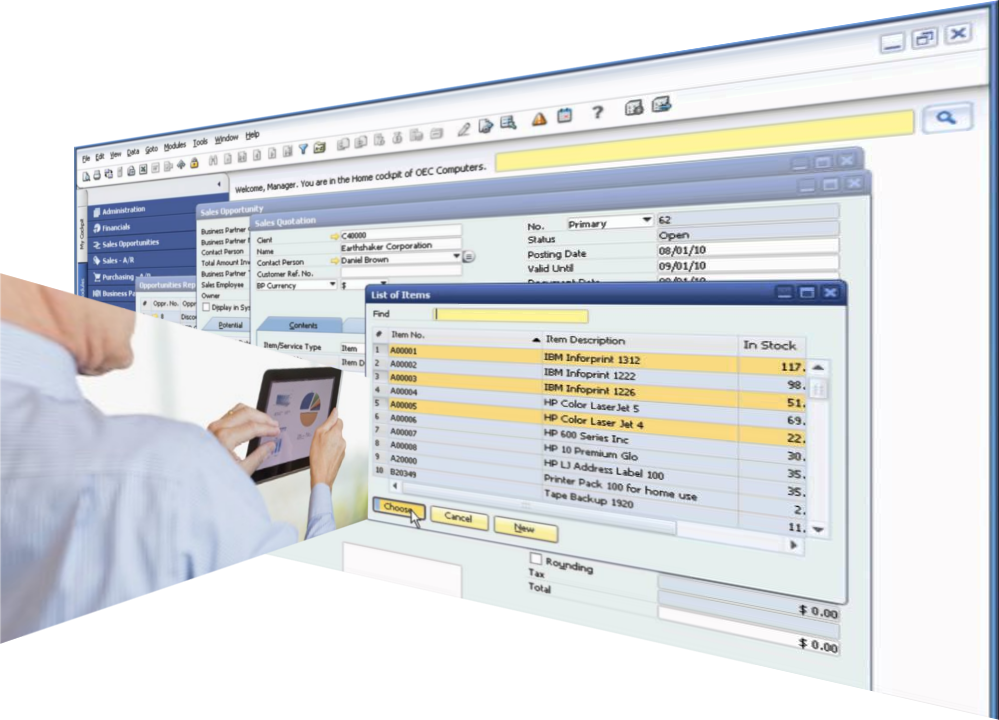
\includegraphics[width=0.7\textwidth]{Images/Titelbild.png}
\label{fig:title}
\end{figure}
% Author and supervisor
\begin{minipage}{0.4\textwidth}
\begin{flushleft} \large
\emph{Autoren:}\\
Marco Moro\\
Severin Gmür\\
Ramon Wyss\\
Tobias Kreienbühl\\
\end{flushleft}
\end{minipage}
\hfill
\begin{minipage}{0.4\textwidth}
\begin{flushright} \large
%\emph{Supervisor:} \\
%tbd
\end{flushright}
\end{minipage}
\large
\vfill
I.BA\_APPE.F1701 \\
Hochschule Luzern Informatik

\end{center}

\end{titlepage}

\tableofcontents
\clearpage


% !TEX root = Dokumentation_SysSpec.tex

\begin{table}[H]
\begin{tabular}{ | p{0.05\textwidth} | p{0.10\textwidth} | p{0.35\textwidth} | p{0.44\textwidth} | }
\hline \rowcolor{gray!50}
%Titelzeile
	\textbf{Rev.} &
	\textbf{Datum}	 	 &
	\textbf{Autor}	 	 &
	\textbf{Bemerkung}
	\\ \hline
%Zeile
	0.1					&
	18.03.17  			&
		Tobias K. \& Marco M.  		&
	\begin{tabular}{l}
		- GitHub \\
		- Entwurf
		im Team
	\end{tabular}
	\\ \hline	%Untere Abgrenzung
%Zeile
	0.2 &
	04.04.17 &
	Severin G. &
	\begin{tabular}{l}
		- Abbildung Use Case
	\end{tabular}
	\\ \hline	%Untere Abgrenzung
%Zeile
	0.3 &
	25.04.17 &
	Alle &
	\begin{tabular}{l}
		- Diverse Anpassungen\\
		- Überarbeitung
	\end{tabular}
	\\ \hline	%Untere Abgrenzung
%Zeile
	0.4 &
	07.05.17 &
	Marco M. &
	\begin{tabular}{l}
		- Ergänzung Entwurfsentscheid\\
		- Definition Environment-Anforderungen\\
		- Ergänzung externe Schnittstellen
	\end{tabular}
	\\ \hline	%Untere Abgrenzung
%Zeile
	0.5 &
	27.05.17 &
	Ramon W. &
	\begin{tabular}{l}
		- Erstellung Ausblick\\
		- Datenmodell
	\end{tabular}
	\\ \hline	%Untere Abgrenzung
\end{tabular}

\label{tab: version}
\caption{Version}
\end{table}

\clearpage

\section{Systemübersicht}


%-------------------
% Systemübersicht
%-------------------
% !TEX root = Dokumentation_SysSpec.tex
\subsection{}

todo


\section{Use Case}
%-------------------
% Use Case
%-------------------
% !TEX root = Dokumentation_SysSpec.tex
\subsection{Use Case Übersicht}
%--------------------------
% Bild Übersicht
%--------------------------

\begin{figure}[H]%Position festigen
\centering
\includegraphics[width=0.7\textwidth]{Images/usecase-u.png}
\label{fig:usecase}
\end{figure}


\subsection{Use Case Beschreibung}
In diesem Abschnitt wird die unter Abbildung 2 dargestellte Use Case Übersichtlich tabellarisch genauer beschrieben.

%--------------------------
%Tabellen usecase/1usecase
%--------------------------
% !TEX root = Dokumentation_SysSpec.tex
\subsubsection{Use Case 1: Anmeldung}
\begin{table}[H]
\begin{tabular}{ | p{0.22\textwidth} | p{0.68\textwidth} |} \hline
\rowcolor{gray!50}
%Titelzeile
	\textbf{Name}          &
	\begin{tabular}{l}
		\textbf{Anmeldung}
	\end{tabular}
	\\ \hline
%Zeile
	\textbf{Kurzbeschreibung}			 &
	\begin{tabular}{l}
		Ein Benutzer meldet sich im System an
	\end{tabular}
\\ \hline
%Zeile
	\textbf{Akteure}}   		 &
	\begin{tabular}{l}
		Filialleiter, Verkaufspersonal, Sysadmin, Filialverwalter, Datatypist
	\end{tabular}
\\ \hline
%Zeile
	\textbf{Auslöser}              & 
	\begin{tabular}{l}
		Der Akteure will sich am System anmelden
	\end{tabular}
\\ \hline
%Zeile
	\textbf{Vorbedingungen}       &
	\begin{tabular}{l}
		-	Der Akteur muss im System vorhanden sein \\
		-	Benutzername muss vorhanden sein \\
		-	Passwort muss vorhanden sein \\

	\end{tabular}		
\\ \hline
%Zeile
	\textbf{Input Information}             &        
	\begin{tabular}{l}
		-	Username \\
		-	Passwort

	\end{tabular}
\\ \hline
%Zeile
	\textbf{Ergebnisse}  &
	\begin{tabular}{l}
		Benutzer ist am System angemeldet.
	\end{tabular}
\\ \hline
%Zeile
	\textbf{Nachbedingung}				 &
	\begin{tabular}{l}
		Benutzer kann im System je nach definierter Rolle arbeiten.
	\end{tabular}
\\ \hline
%Zeile
	\textbf{Ablauf}            &
	\begin{tabular}{l}
		1.	Applikation starten \\
		2.	Username \& Passwort eingeben \\
		3.	Schaltfläche \glqq{} \«Login\»\grqq{} betätigen

	\end{tabular}
\\ \hline
%Zeile
	\textbf{Sonderfälle}			 &
	\begin{tabular}{l}
		Passwort wird 3-mal falsch eingegeben.
	\end{tabular}
\\ \hline	
%Untere Abgrenzung
\end{tabular}
\end{table}
% !TEX root = Dokumentation_SysSpec.tex
\subsubsection{Use Case 2:Bestellung einsehen }
\begin{table}[H]
\begin{tabular}{ | p{0.22\textwidth} | p{0.68\textwidth} |} \hline
\rowcolor{gray!50}
%Titelzeile
	\textbf{Name}          &
	\begin{tabular}{l}
		\textbf{Bestellung einsehen}
	\end{tabular}
	\\ \hline
%Zeile
	\textbf{Kurzbeschreibung}			 &
	\begin{tabular}{l}
		Akteure kann sich alle offenen Bestellungen ansehen.
	\end{tabular}
\\ \hline
%Zeile
	\textbf{Akteure}   		 &
	\begin{tabular}{l}
		Filialleiter, Verkaufspersonal
	\end{tabular}
\\ \hline
%Zeile
	\textbf{Auslöser}              & 
	\begin{tabular}{l}
		Ein Akteure will die Bestellungen einsehen.
	\end{tabular}
\\ \hline
%Zeile
	\textbf{Vorbedingungen}       &
	\begin{tabular}{l}
		-	Der Akteur muss im System angemeldet sein
	
	\end{tabular}		
\\ \hline
%Zeile
	\textbf{Input Information}             &        
	\begin{tabular}{l}
		-	Auswahl aus Liste.

	\end{tabular}
\\ \hline
%Zeile
	\textbf{Ergebnisse}  &
	\begin{tabular}{l}
		Bestellung wird angezeigt.
	\end{tabular}
\\ \hline
%Zeile
	\textbf{Nachbedingung}				 &
	\begin{tabular}{l}
		-
	\end{tabular}
\\ \hline
%Zeile
	\textbf{Ablauf}            &
	\begin{tabular}{l}
		1.	Bestellung aus Liste auswählen. \\
		2.	Doppelklick auf anzuzeigende Bestellung.

	\end{tabular}
\\ \hline
%Zeile
	\textbf{Sonderfälle}			 &
	\begin{tabular}{l}
		-
	\end{tabular}
\\ \hline	
%Untere Abgrenzung
\end{tabular}
\label{tab:2usecase}
\caption{Use Case 2: Bestellung einsehen}
\end{table}
% !TEX root = Dokumentation_SysSpec.tex
\subsubsection{Use Case 3: Bestellung erfassen}
\begin{table}[H]
\begin{tabular}{ | p{0.22\textwidth} | p{0.68\textwidth} |} \hline
\rowcolor{gray!50}
%Titelzeile
	\textbf{Name}          &
	\begin{tabular}{l}
		\textbf{Bestellung erfassen}
	\end{tabular}
	\\ \hline
%Zeile
	\textbf{Kurzbeschreibung}			 &
	\begin{tabular}{l}
		Ein Akteure erfasst aus den bestehenden Produkten eine Bestellungen.
	\end{tabular}
\\ \hline
%Zeile
	\textbf{Akteure}   		 &
	\begin{tabular}{l}
		Filialleiter, Verkaufspersonal
	\end{tabular}
\\ \hline
%Zeile
	\textbf{Auslöser}              & 
	\begin{tabular}{l}
		Kunde möchte via Akteure ein Produkt bestellen.
	\end{tabular}
\\ \hline
%Zeile
	\textbf{Vorbedingungen}       &
	\begin{tabular}{l}
		-	Der Akteur muss im System angemeldet sein (Use Case 1 erfüllt).\\
		-	Der Akteur ist berechtige Bestellungen zu erfassen. \\
		- 	Der Kunde muss bereits im System erfasst sein \\
		- 	Das Produkt muss in der Datenbank (Filliallager) vorhanden sein. 
  

	\end{tabular}		
\\ \hline
%Zeile
	\textbf{Input Information}             &        
	\begin{tabular}{l}
		
		-   Kunde \\
		-	Produkt \\
		-  	Anzahl 
		

	\end{tabular}
\\ \hline
%Zeile
	\textbf{Ergebnisse}  &
	\begin{tabular}{l}
		Verkäufer erfasst von Kunde gewünschte Produkte.
	\end{tabular}
\\ \hline
%Zeile
	\textbf{Nachbedingung}				 &
	\begin{tabular}{l}
		Wenn Bestellung erfasst ist, wird Rechnungswesen benachrichtigt \& \\
		der Kunde erhält eine Bestellbestätigung.
	\end{tabular}
\\ \hline
%Zeile
	\textbf{Ablauf}            &
	\begin{tabular}{l}
		1.	Verkäufer ist am System angemeldet. \\
		2.	Kunde auswählen (Dropdown List). \\
		3.  Produkt in Liste suchen und Anzahl eingeben.\\
		4.  Falls mehrere Produkte gewünscht werden, Schritt 3 wiederholen.\\
		5.	Schaltfläche \grqq Bestellung absenden\grqq{} betätigen. \\
		
	

	\end{tabular}
\\ \hline
%Zeile
	\textbf{Sonderfälle}			 &
	\begin{tabular}{l}
		- Kunde hat offene Mahnung -> Bei der Kundenansicht eine Info.\\
		- Produkt ist unter Lagerbestand -> Nachbestellung auslösen\\
		- Wenn Kunde während Bestellung keine Produkt mehr möchte \\
		  -> Schaltfläche \grqq abbrechen\grqq{}  betätigen. \\
		- Bestellung absenden ohne Produktanzahl eingegeben -> Nullwert Übergabe 
	\end{tabular}
\\ \hline	
%Untere Abgrenzung
\end{tabular}
\label{tab:3usecase}
\caption{Use Case 3: Bestellung erfassen}
\end{table}
% !TEX root = Dokumentation_SysSpec.tex
\subsubsection{Use Case 4: Bestellung bearbeiten}
\begin{table}[H]
\begin{tabular}{ | p{0.22\textwidth} | p{0.68\textwidth} |} \hline
\rowcolor{gray!50}
%Titelzeile
	\textbf{Name}          &
	\begin{tabular}{l}
		\textbf{Bestellung bearbeiten}
	\end{tabular}
	\\ \hline
%Zeile
	\textbf{Kurzbeschreibung}			 &
	\begin{tabular}{l}
		Ein Akteure kann Bestellungen ändern oder annullieren.
	\end{tabular}
\\ \hline
%Zeile
	\textbf{Akteure}   		 &
	\begin{tabular}{l}
		Filialleiter, Verkaufspersonal
	\end{tabular}
\\ \hline
%Zeile
	\textbf{Auslöser}              & 
	\begin{tabular}{l}
		Eine Bestellung wird bearbeitet.
	\end{tabular}
\\ \hline
%Zeile
	\textbf{Vorbedingungen}       &
	\begin{tabular}{l}
		-	Der Akteur muss im System angemeldet sein (Use Case 1 erfüllt).\\
		-	Der Akteur ist berechtige Bestellungen zu bearbeiten. \\		
		- 	Eine Bestellung muss vorhanden sein. \\
  

	\end{tabular}		
\\ \hline
%Zeile
	\textbf{Input Information}             &        
	\begin{tabular}{l}

		-   Bestellinformationen 
		
		

	\end{tabular}
\\ \hline
%Zeile
	\textbf{Ergebnisse}  &
	\begin{tabular}{l}
		Akteur ändert oder annulliert eine Bestellung.
	\end{tabular}
\\ \hline
%Zeile
	\textbf{Nachbedingung}				 &
	\begin{tabular}{l}
		- Akteur kann die geänderte Bestellung einsehen.\\
		- Rechnungswesen wird benachrichtigt.\\
		- Kunde bekommt neue Bestellbestätigung.
	\end{tabular}
\\ \hline
%Zeile
	\textbf{Ablauf}            &
	\begin{tabular}{l}
		1.	Akteur ist am System angemeldet (Use Case 1 ist erfüllt). \\
		2.	Bestellung aus Liste auswählen. \\
		3.	Schaltfläche \grqq Bestellung annotieren\grqq{} betätigen \\
			um Bestellung zu löschen.\\
		4. 	Schaltfläche \grqq Bestellung editieren\grqq{} betätigen \\
			um Bestellung zu ändern.\\
		5.	Liste mit Bestellungen wird angezeigt \\
		6.	Anzahl der Produkte anpassen\\
		7.  Schaltfläche \grqq Bestellung absenden\grqq{}  betätigen.

	\end{tabular}
\\ \hline
%Zeile
	\textbf{Sonderfälle}			 &
	\begin{tabular}{l}
		- Kunde hat offene Mahnung -> Bei der Kundenansicht eine Info.\\
		- Produkt ist unter Lagerbestand -> Nachbestellung auslösen\\
		- Wenn Kunde während Bestellung keine Produkt mehr möchte \\
		       -> Schaltfläche \grqq abbrechen\grqq{}  betätigen. \\
		- Bestellung abs. ohne Produktanzahl eingeb. -> Nullwert Übergabe 
	\end{tabular}
\\ \hline	
%Untere Abgrenzung
\end{tabular}
\label{tab:4usecase}
\caption{Use Case 4: Bestellung bearbeiten}
\end{table}
% !TEX root = Dokumentation_SysSpec.tex
\subsubsection{Use Case 5: }
\begin{table}[H]
\begin{tabular}{ | p{0.22\textwidth} | p{0.68\textwidth} |} \hline
\rowcolor{gray!50}
%Titelzeile
	\textbf{Name}          &
	\begin{tabular}{l}
		\textbf{Wareineingang erfassen}
	\end{tabular}
	\\ \hline
%Zeile
	\textbf{Kurzbeschreibung}			 &
	\begin{tabular}{l}
		Wenn eine Ware eintrifft wird sie vom Datentypist erfasst.
	\end{tabular}
\\ \hline
%Zeile
	\textbf{Akteure}   		 &
	\begin{tabular}{l}
		Datatypist
	\end{tabular}
\\ \hline
%Zeile
	\textbf{Auslöser}              & 
	\begin{tabular}{l}
		Ware wird geliefert.
	\end{tabular}
\\ \hline
%Zeile
	\textbf{Vorbedingungen}       &
	\begin{tabular}{l}
		-	Der Akteur muss im System angemeldet sein.
		 

	\end{tabular}		
\\ \hline
%Zeile
	\textbf{Input Information}             &        
	\begin{tabular}{l}
		-	Ware wird an Filiale geliefert

	\end{tabular}
\\ \hline
%Zeile
	\textbf{Ergebnisse}  &
	\begin{tabular}{l}
		Filialager wird benachrichtigt.
	\end{tabular}
\\ \hline
%Zeile
	\textbf{Nachbedingung}				 &
	\begin{tabular}{l}
		Ware wird an Kunde ausgeliefert oder abgeholt.
	\end{tabular}
\\ \hline
%Zeile
	\textbf{Ablauf}            &
	\begin{tabular}{l}
		1.	Ware im System erfassen \\
		2.	Kunde benachrichtigen \\
		

	\end{tabular}
\\ \hline
%Zeile
	\textbf{Sonderfälle}			 &
	\begin{tabular}{l}
		- Ware kommt nicht vollständig zur Filiale -> Teillieferung \\oder auf komplett Ware warten. \\
		- Defektes oder unvollständige Lieferung -> Zurück an Filiallager.
	\end{tabular}
\\ \hline	
%Untere Abgrenzung
\end{tabular}
\end{table}
% !TEX root = Dokumentation_SysSpec.tex
\subsubsection{Use Case 6: }
\begin{table}[H]
\begin{tabular}{ | p{0.22\textwidth} | p{0.68\textwidth} |} \hline
\rowcolor{gray!50}
%Titelzeile
	\textbf{Name}          &
	\begin{tabular}{l}
		\textbf{Anmeldung}
	\end{tabular}
	\\ \hline
%Zeile
	\textbf{Kurzbeschreibung}			 &
	\begin{tabular}{l}
		Ein Benutzer meldet sich im System an
	\end{tabular}
\\ \hline
%Zeile
	\textbf{Akteure}   		 &
	\begin{tabular}{l}
		Filialleiter, Verkaufspersonal, Sysadmin, Filialverwalter, Datatypist
	\end{tabular}
\\ \hline
%Zeile
	\textbf{Auslöser}              & 
	\begin{tabular}{l}
		Der Akteure will sich am System anmelden
	\end{tabular}
\\ \hline
%Zeile
	\textbf{Vorbedingungen}       &
	\begin{tabular}{l}
		-	Der Akteur muss im System vorhanden sein \\
		-	Benutzername muss vorhanden sein \\
		-	Passwort muss vorhanden sein 

	\end{tabular}		
\\ \hline
%Zeile
	\textbf{Input Information}             &        
	\begin{tabular}{l}
		-	Username \\
		-	Passwort

	\end{tabular}
\\ \hline
%Zeile
	\textbf{Ergebnisse}  &
	\begin{tabular}{l}
		Benutzer ist am System angemeldet.
	\end{tabular}
\\ \hline
%Zeile
	\textbf{Nachbedingung}				 &
	\begin{tabular}{l}
		Benutzer kann im System je nach definierter Rolle arbeiten.
	\end{tabular}
\\ \hline
%Zeile
	\textbf{Ablauf}            &
	\begin{tabular}{l}
		1.	Applikation starten \\
		2.	Username \& Passwort eingeben \\
		3.	Schaltfläche Login betätigen

	\end{tabular}
\\ \hline
%Zeile
	\textbf{Sonderfälle}			 &
	\begin{tabular}{l}
		Passwort wird 3-mal falsch eingegeben.
	\end{tabular}
\\ \hline	
%Untere Abgrenzung
\end{tabular}
\end{table}
% !TEX root = Dokumentation_SysSpec.tex
\subsubsection{Use Case 7: Nachbestellung auslösen}
\begin{table}[H]
\begin{tabular}{ | p{0.22\textwidth} | p{0.68\textwidth} |} \hline
\rowcolor{gray!50}
%Titelzeile
	\textbf{Name}          &
	\begin{tabular}{l}
		\textbf{Nachbestellung auslösen}
	\end{tabular}
	\\ \hline
%Zeile
	\textbf{Kurzbeschreibung}			 &
	\begin{tabular}{l}
		Der Lagerbestand wird mit dem definierten Grenzwert verglichen und eine Bestellung ausgelöst.
	\end{tabular}
\\ \hline
%Zeile
	\textbf{Akteure}   		 &
	\begin{tabular}{l}
		- 
	\end{tabular}
\\ \hline
%Zeile
	\textbf{Auslöser}              & 
	\begin{tabular}{l}
		Lagerbestand ist unter den definierten Grenzwert gefallen.
	\end{tabular}
\\ \hline
%Zeile
	\textbf{Vorbedingungen}       &
	\begin{tabular}{l}
		-	Bestellung wird abgeschlossen.

	\end{tabular}		
\\ \hline
%Zeile
	\textbf{Input Information}             &        
	\begin{tabular}{l}
		-	Lagerbestand. \\
		-   Bestand Nachbestellung. \\
		-	Definierter Grenzwert.\\

	\end{tabular}
\\ \hline
%Zeile
	\textbf{Ergebnisse}  &
	\begin{tabular}{l}
		Nachbestellung wird ausgelöst.
	\end{tabular}
\\ \hline
%Zeile
	\textbf{Nachbedingung}				 &
	\begin{tabular}{l}
		- 
	\end{tabular}
\\ \hline
%Zeile
	\textbf{Ablauf}            &
	\begin{tabular}{l}
		1.  Bestellung wird ausgelöst.\
		2.	Lagerbestand von Artikel. \\
		3.	Vergleich mit definierten Grenzwert. \\
		4.	Prüfen ob Nachbestellung aktiv.

	\end{tabular}
\\ \hline
%Zeile
	\textbf{Sonderfälle}			 &
	\begin{tabular}{l}
		- Lagerbestand ist über minimalen Lagerbestand -> keine Nachbestellung auslösen.
	\end{tabular}
\\ \hline	
%Untere Abgrenzung
\end{tabular}
\label{tab:7usecase}
\caption{Use Case 7: Nachbestellung auslösen}
\end{table}
% !TEX root = Dokumentation_SysSpec.tex
\subsubsection{Use Case 8: }
\begin{table}[H]
\begin{tabular}{ | p{0.22\textwidth} | p{0.68\textwidth} |} \hline
\rowcolor{gray!50}
%Titelzeile
	\textbf{Name}          &
	\begin{tabular}{l}
		\textbf{Nachbestellung einsehen}
	\end{tabular}
	\\ \hline
%Zeile
	\textbf{Kurzbeschreibung}			 &
	\begin{tabular}{l}
		Filialleiter kann die Nachbestellungen einsehen.
	\end{tabular}
\\ \hline
%Zeile
	\textbf{Akteure}   		 &
	\begin{tabular}{l}
		Filialleiter
	\end{tabular}
\\ \hline
%Zeile
	\textbf{Auslöser}              & 
	\begin{tabular}{l}
		Filialleiter will Nachbestellungen ansehen.
	\end{tabular}
\\ \hline
%Zeile
	\textbf{Vorbedingungen}       &
	\begin{tabular}{l}
		-	Der Akteur muss im System angemeldet sein (Use Case 1 erfüllt). \\


	\end{tabular}		
\\ \hline
%Zeile
	\textbf{Input Information}             &        
	\begin{tabular}{l}
		-	Liste Nachbestellung Zentrallager
	\end{tabular}
\\ \hline
%Zeile
	\textbf{Ergebnisse}  &
	\begin{tabular}{l}
		Nachbestellungen werden aufgelistet.
	\end{tabular}
\\ \hline
%Zeile
	\textbf{Nachbedingung}				 &
	\begin{tabular}{l}
		-
	\end{tabular}
\\ \hline
%Zeile
	\textbf{Ablauf}            &
	\begin{tabular}{l}
		1.	Schaltfläche \grqq Nachbestellungen\grqq{} betätigen. \\
		2.	Produkt in Liste auswählen. \\
		3.	Schaltfläche \grqq Anzeigen\grqq{} betätigen.

	\end{tabular}
\\ \hline
%Zeile
	\textbf{Sonderfälle}			 &
	\begin{tabular}{l}
		- Es wird eine leere Liste angezeigt wenn keine Nachbestellungen ausgelöst worden sind.
	\end{tabular}
\\ \hline	
%Untere Abgrenzung
\end{tabular}
\label{tab:8usecase}
\caption{Use Case 8: Nachbestellung einsehen}
\end{table}





\section{Architektur und Designentscheide}
%-------------------
% Systemübersicht
%-------------------
% !TEX root = Dokumentation_SysSpec.tex
\subsection{Modelle und Sichten}

\subsubsection{Kontextdiagramm}
Die entwickelte Applikation hat folgende Abhängigkeiten/Umsysteme/Akteuere:
\begin{figure}[H]
	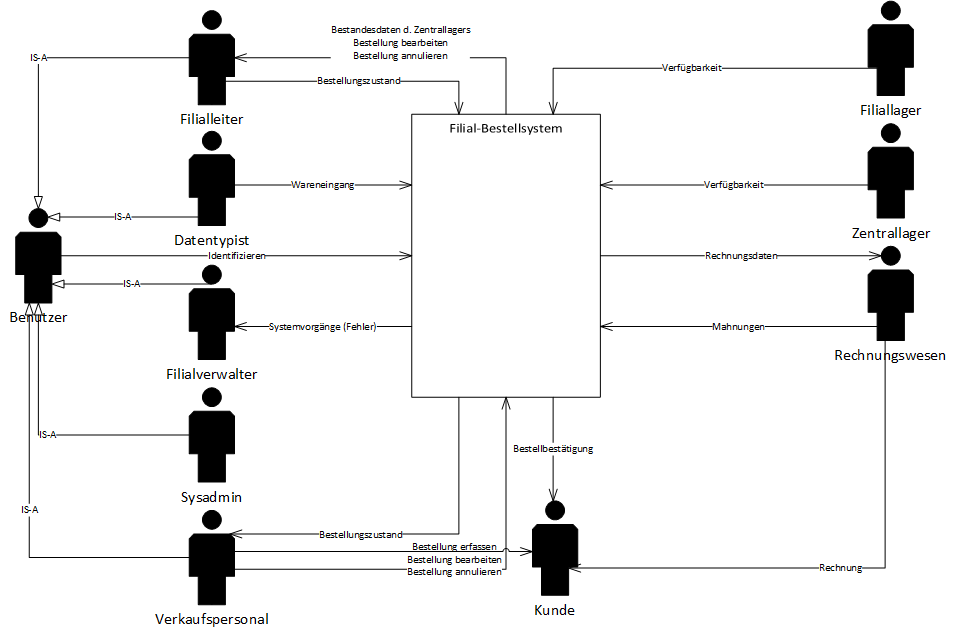
\includegraphics[width=1.0\linewidth]{Images/kontextdiagram}
	\caption{Kontextdiagram}
	\label{fig:kontextdiagram}
\end{figure}

\textbf{Umsysteme}:
\begin{itemize}
\item Zentrallager: Nachbestellungen des lokalen Filiallagers werden an das Zentrallager gesendet.
\item Rechnungswesen: Das Rechnungswesen wird für Bestell-Bestätigungen, Rechnungsversand und Mahnungsprüfungen verwendet.
\item Filiallager: Lagerung der in der Filiale verkauften Artikel. Filiallager und Applikation müssen jederzeit einen übereinstimmenden Datenbestand haben.
\end{itemize}

\textbf{Akteuere}:
\begin{itemize}
\item Benutzer: Bestehend aus Filialverwalter, Filialleiter, Verkaufspersonal und Datentypist, bezeichnet alle Nutzer der Applikation. Die einzelnen Aktionen sind in der Use Case Übersicht ersichtlich
\item Sysadmin: Gemäss Anforderungen kein eigentlicher Benutzer. Für konfigurative Anpassungen könnte ein Zugriff notwendig sein
\item Kunde: Interaktion mit der Applikation wird via Verkaufspersonal abgewickelt.
\end{itemize}


\subsubsection{Layer-Architektur}
TODO Übersichsgrafik importieren und erläutern

\subsubsection{Client-Layer}
Der Client-Layer ist in JavaFX implementiert und verwendet das MVC-Architektur-Pattern. Zur Gestaltung der Oberfläche wurde ein 3rd Party Tool eingesetzt, um die graphische Gestaltung zu vereinfachen.
\begin{itemize}
\item Scene Builder by Gluon: Basiert auf der von Oracle entwickelten JavaFX-Distribution, und erstellt ein passendes FXML-Dokument für die Einbindung der graphischen Oberfläche, inklusive Verlinkung und definition der Event-Handler. 
\end{itemize}
\begin{figure}[H]
	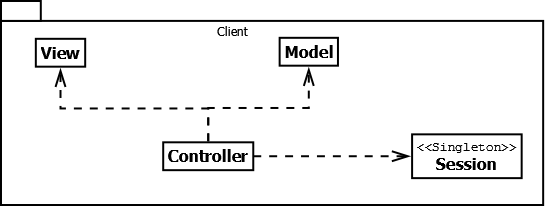
\includegraphics[width=1.0\linewidth]{Images/ClientLayer-Architektur}
	\caption{Architektur des Clientlayer}
	\label{fig:clientlayer-architektur}
\end{figure}

\textbf{View}: Die View ist dafür verantwortlich, dass die angezeigte Oberfläche korrekt geladen ist.

\textbf{Controller}: Die Controller binden die FXML-Dokumente ein. Die Controller registrieren ausgelöste Events und steuern die durchzufürenden Aktionen, wie Datenabfragen vom Business-Layer durch.

\textbf{Model}: Im Model befinden sich die im GUI angezeigten Datenwerte, und sind bereits durch die Verwendung von Property-Klassen als Observable-Objekte abgespeichert.

\textbf{Session}: Die Session enthält die User-Informationen. Die Session-Informationen werden bei Aktionen mitgesendet, um unauthorisierte Aufrufe zu unterbinden.

\subsubsection{Remote-Layer}
\begin{figure}[H]
	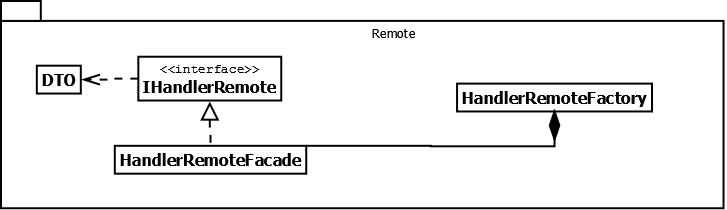
\includegraphics[width=1.0\linewidth]{Images/RemoteLayer-Architektur}
	\caption{Architektur des Remotelayer}
	\label{fig:remotelayer-architektur}
\end{figure}

\subsubsection{Business-Layer}
\begin{figure}[H]
	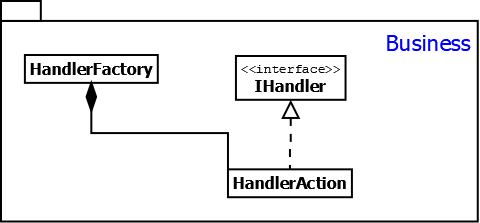
\includegraphics[width=1.0\linewidth]{Images/BusinessLayer-Architektur}
	\caption{Architektur des Businesslayer}
	\label{fig:businesslayer-architektur}
\end{figure}

\subsubsection{Data-Layer}
\begin{figure}[H]
	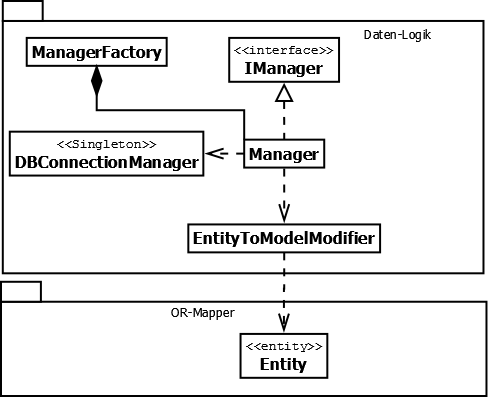
\includegraphics[width=1.0\linewidth]{Images/DataLayer-Architektur}
	\caption{Architektur des Datalayer}
	\label{fig:datalayer-architektur}
\end{figure}

\subsubsection{UML-Klassendiagramme}
todo


\subsubsection{Sequenzdiagramme}
todo


\subsection{Entwurfsentscheid}
Im Rahmen der Architekturausarbeitung wurden folgende Entwurfsentscheide gefällt:
\begin{itemize}
	\item Für Testzwecke und statische Datenstrukturen werden teilweise Stubs eingesetzt. Beispielsweise sind die Zuweisung Benutzerrollen zu deren Berechtigungen bis Release 1.0 als Stub abgebildet.
	\item Der Business-Layer und Data-Layer (ohne Datenbank, nur OR-Mapper) befinden sich auf dem gleichen Tier. Bis Release 1.0 werden, aus zeitlichen Gründen, keine Bestrebungen zur Aufteilung dieser Layers auf verschiedene Tiers vorgenommen
	\item Die Tier-übergreifende Kommunikation zwischen Tier Client und Business wird mittels RMI (Remote Method Invocation) umgesetzt. Eine alternative Anbindung bspw. mit REST (Representational state transfer) wird nach Release 1.0 in Betracht gezogen.
	\item Als GUI-Komponente auf Layer Client wird JavaFX verwendet.
	\item Als Datenbank wird eine MySQL-Instanz aus dem EnterpriseLab der HSLU verwendet.
	\item Bis Release 1.0 müssen neue Kunden \& Artikel in der Datenbank manuell erfasst / abgebildet werden. Diese werden idealerweise mit einer zentralen Benutzerverwaultung (Rechnungswesen, Zentrallager) in folgenden Releases zusammengeführt.
	\item Die Rechnungsdaten und Mahnungen werden aufgrund in einem Stub generiert. Die Anbindung eines beliebigen, externen Rechnungswesen ist dadurch in folgenden Releases schneller zu bewältigen.
\end{itemize}

TODO
- Dateien einbinden (DB) -> Transaktionsmanagement


\subsection{Datenmodell}
Der Aufbau der Datenbank ist in folgender Abbildung dargestellt.
\begin{figure}[H]
	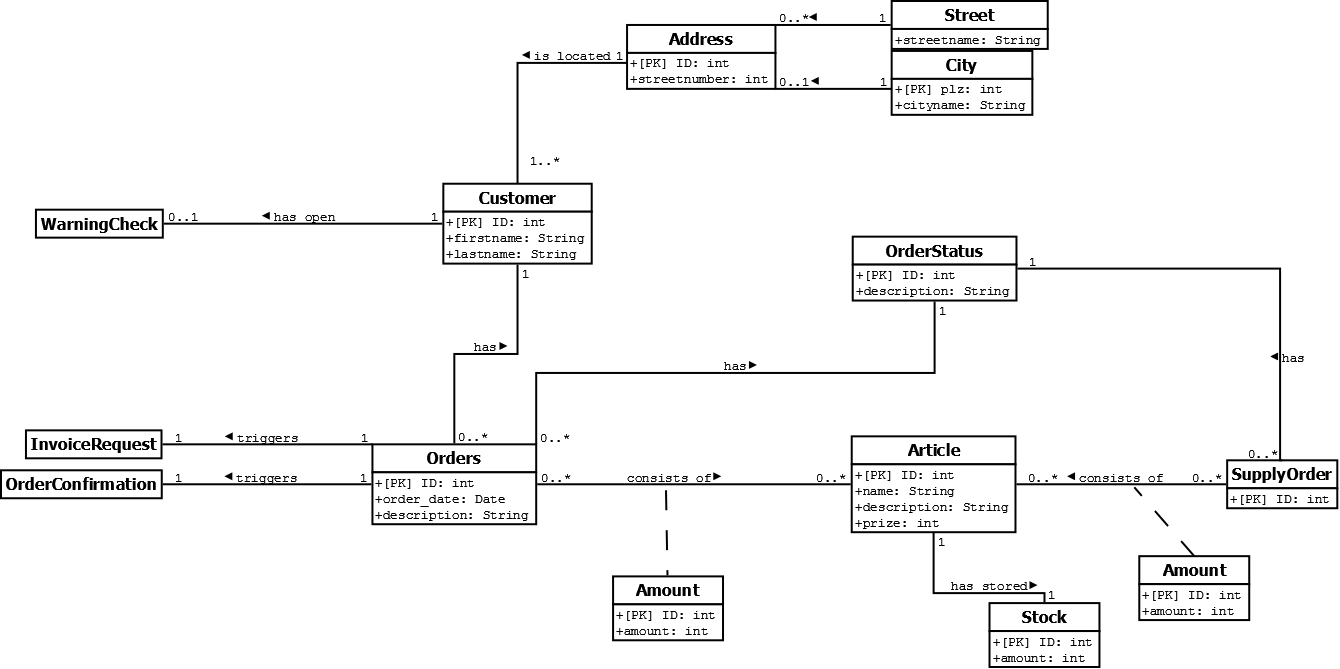
\includegraphics[width=1.0\linewidth]{Images/datamodel}
	\caption{Datenmodel}
	\label{fig:datamodel}
\end{figure}
Die Datenbank ist funktional aufgebaut und befolgt die ersten 3 Normalformen. Die Anbindung von Umsystemen sind im Datenmodell bereits abgebildet, sind jedoch nicht in der Datenbank vorhanden. Die abgebildeten Umsysteme sind WarningCheck, InvoiceRequest und OrderConfirmation.



\section{Schnittstellen}
%-------------------
% Schnittstellen
%-------------------
% !TEX root = Dokumentation_SysSpec.tex
\subsection{Externe Schnittstellen}
\subsubsection{Rollen und Akteure}
Im Rahmen des Filial-Bestellsystems existieren folgende Akteure, welche zugleich spezifische Rollen und somit Berechtigungen besitzen.
\begin{itemize}
	\item Benutzer: Jeder Akteur in der Rolle 'Benutzer' kann sich am System mit den entsprechenden Zugangsdaten anmelden.
	\item Filialleiter: besitzt die Rechte 'OrderView' und 'OrderEdit' und kann daher sowohl bestehende Bestellungen einsehen, bearbeiten und annullieren.
	\item Verkaufspersonal: hat grundsätzlich identische Rechte wie Filialleiter, kann jedoch zusätzlich noch Bestellungen erfassen. TODO: Prüfen, ob wirklich so umgesetzt!
	\item Datentypist: besitzt die Rolle 'Supply' und kann dadurch den Wareneingang im System erfassen
	\item Filialverwalter: besitzt die Rolle 'LogView' und kann daher das Logfile mit den abgelaufenen Systemabläufen überprüfen. Die Einsicht via Filial-Bestellsystem in das Logfile ist nicht im Release 1.0 realisiert. In folgenden Releases wird über eine zentrale Logfile-Verwaltung (bspw. Syslog) entschieden. 
	\item Sysadmin: hat keine aktiven Steuerungsmöglichkeiten innerhalb des Systems. Der Anwendungsfall des Sysadmins ist für Release 1.0 noch nicht definiert.
\end{itemize}
\subsubsection{Datenbankanbindung}
TODO Tobias: OR-Mapper Anbindung beschreiben\\

Für die Persistierung der Daten (ausser Logdaten, RW und Zentrallager) wird eine MySQL-Datenbank aus dem EnterpriseLab mit dem folgenden ConnectionString verwendet:
- TODO ConnectionString
Auf Stufe Datenbank wurden keine weiteren Sichten, Prozeduren und Benutzer eingesetzt. Daher wird gegenüber der Datenbank nur der User grp13 verwendet.
\subsubsection{Zentrallager}
Für das Zentrallager wird eine Stock-Schnittstelle zur Verfügung gestellt. Sie ist in einem Maven-Repo ('https://bintray.com/hslu/maven/appe/5.0.1\#files/ch/hslu/appe/appe\_stock') abgelegt und bereits in das Modul 'appe\_layer\_business' integriert.\\
Die detaillierte Dokumentation zur vorgegebenen Schnittstelle ist unter\\
'https://elearning.hslu.ch/ilias/ilias.php?ref\_id=3290529\&page=APPE\_Startseite\&wpg\_id=11071\&cmd=downloadFile\&cmdClass=ilwikipagegui\&cmdNode=yi:l5:yk\&baseClass=ilwikihandlergui\&file\_id=il\_\_file\_3582976' zu beziehen.

Die Implementation wurde im Business-Layer vorgenommen. Die vorgegebene Schnittstelle wurde nur in einem minimalen Ausmass verwendet. Im Rahmen einer Bestelländerung /-erfassung wird bei Unterschreiten der definierten Mindestanzahl eines Artikels (bis Release 1.0 fix auf 2 definiert) über die Methode 'orderArticle(....)' eine Nachbestellung in der Höhe der geforderten Artikel + 2 ausgelöst. Es wird dabei nicht geprüft, ob am Zentrallager noch entsprechende Artikel vorhanden sind. \\Es wird daher davon ausgegangen, dass am Zentrallager wie auch im Filiallager ein Negativlagerbestand möglich ist. Die Schnittstelle ist dadurch nur unidirektional und es werden keine Daten \& Interaktionen durch das Zentrallager an das Filial-Bestellsystem direkt ausgeführt.  \\
TODO Severin: Klassendiagram hinzufügen
\subsubsection{Rechnungswesen}
Das Rechnungswesen hat die Aufgabe bei Erfassung / Änderung einer Bestellung eine entsprechende Rechnung an den Kunden zu versenden.\\
Von Seiten Auftraggeber sind keine Schnittstellen zur Verfügung gestellt worden und daher wurden die entsprechenden Aufgaben des Rechnungswesen als simpler Stub implementiert, der lediglich ein Output über die ausgeführte Arbeit (z.B. Neue Rechnung gedruckt) protokolliert. \\
TODO Severin: Klassendiagram hinzufügen

\subsection{Interne Schnittstellen}
In diesem Kapitel werden nur wichtige, systemrelevante Schnittstellen spezifiziert. Es werden primär die Schnittstellen zwischen den Layern 'Client', 'Business' inkl. Remote und 'Data' beschrieben.

\subsubsection{Globale Sicht}
In einer groben Übersicht wird die globale Sicht der Schnittstellen zwischen den Schichten / Packages aufgezeigt.:\\
\begin{figure}[H]
\centering
	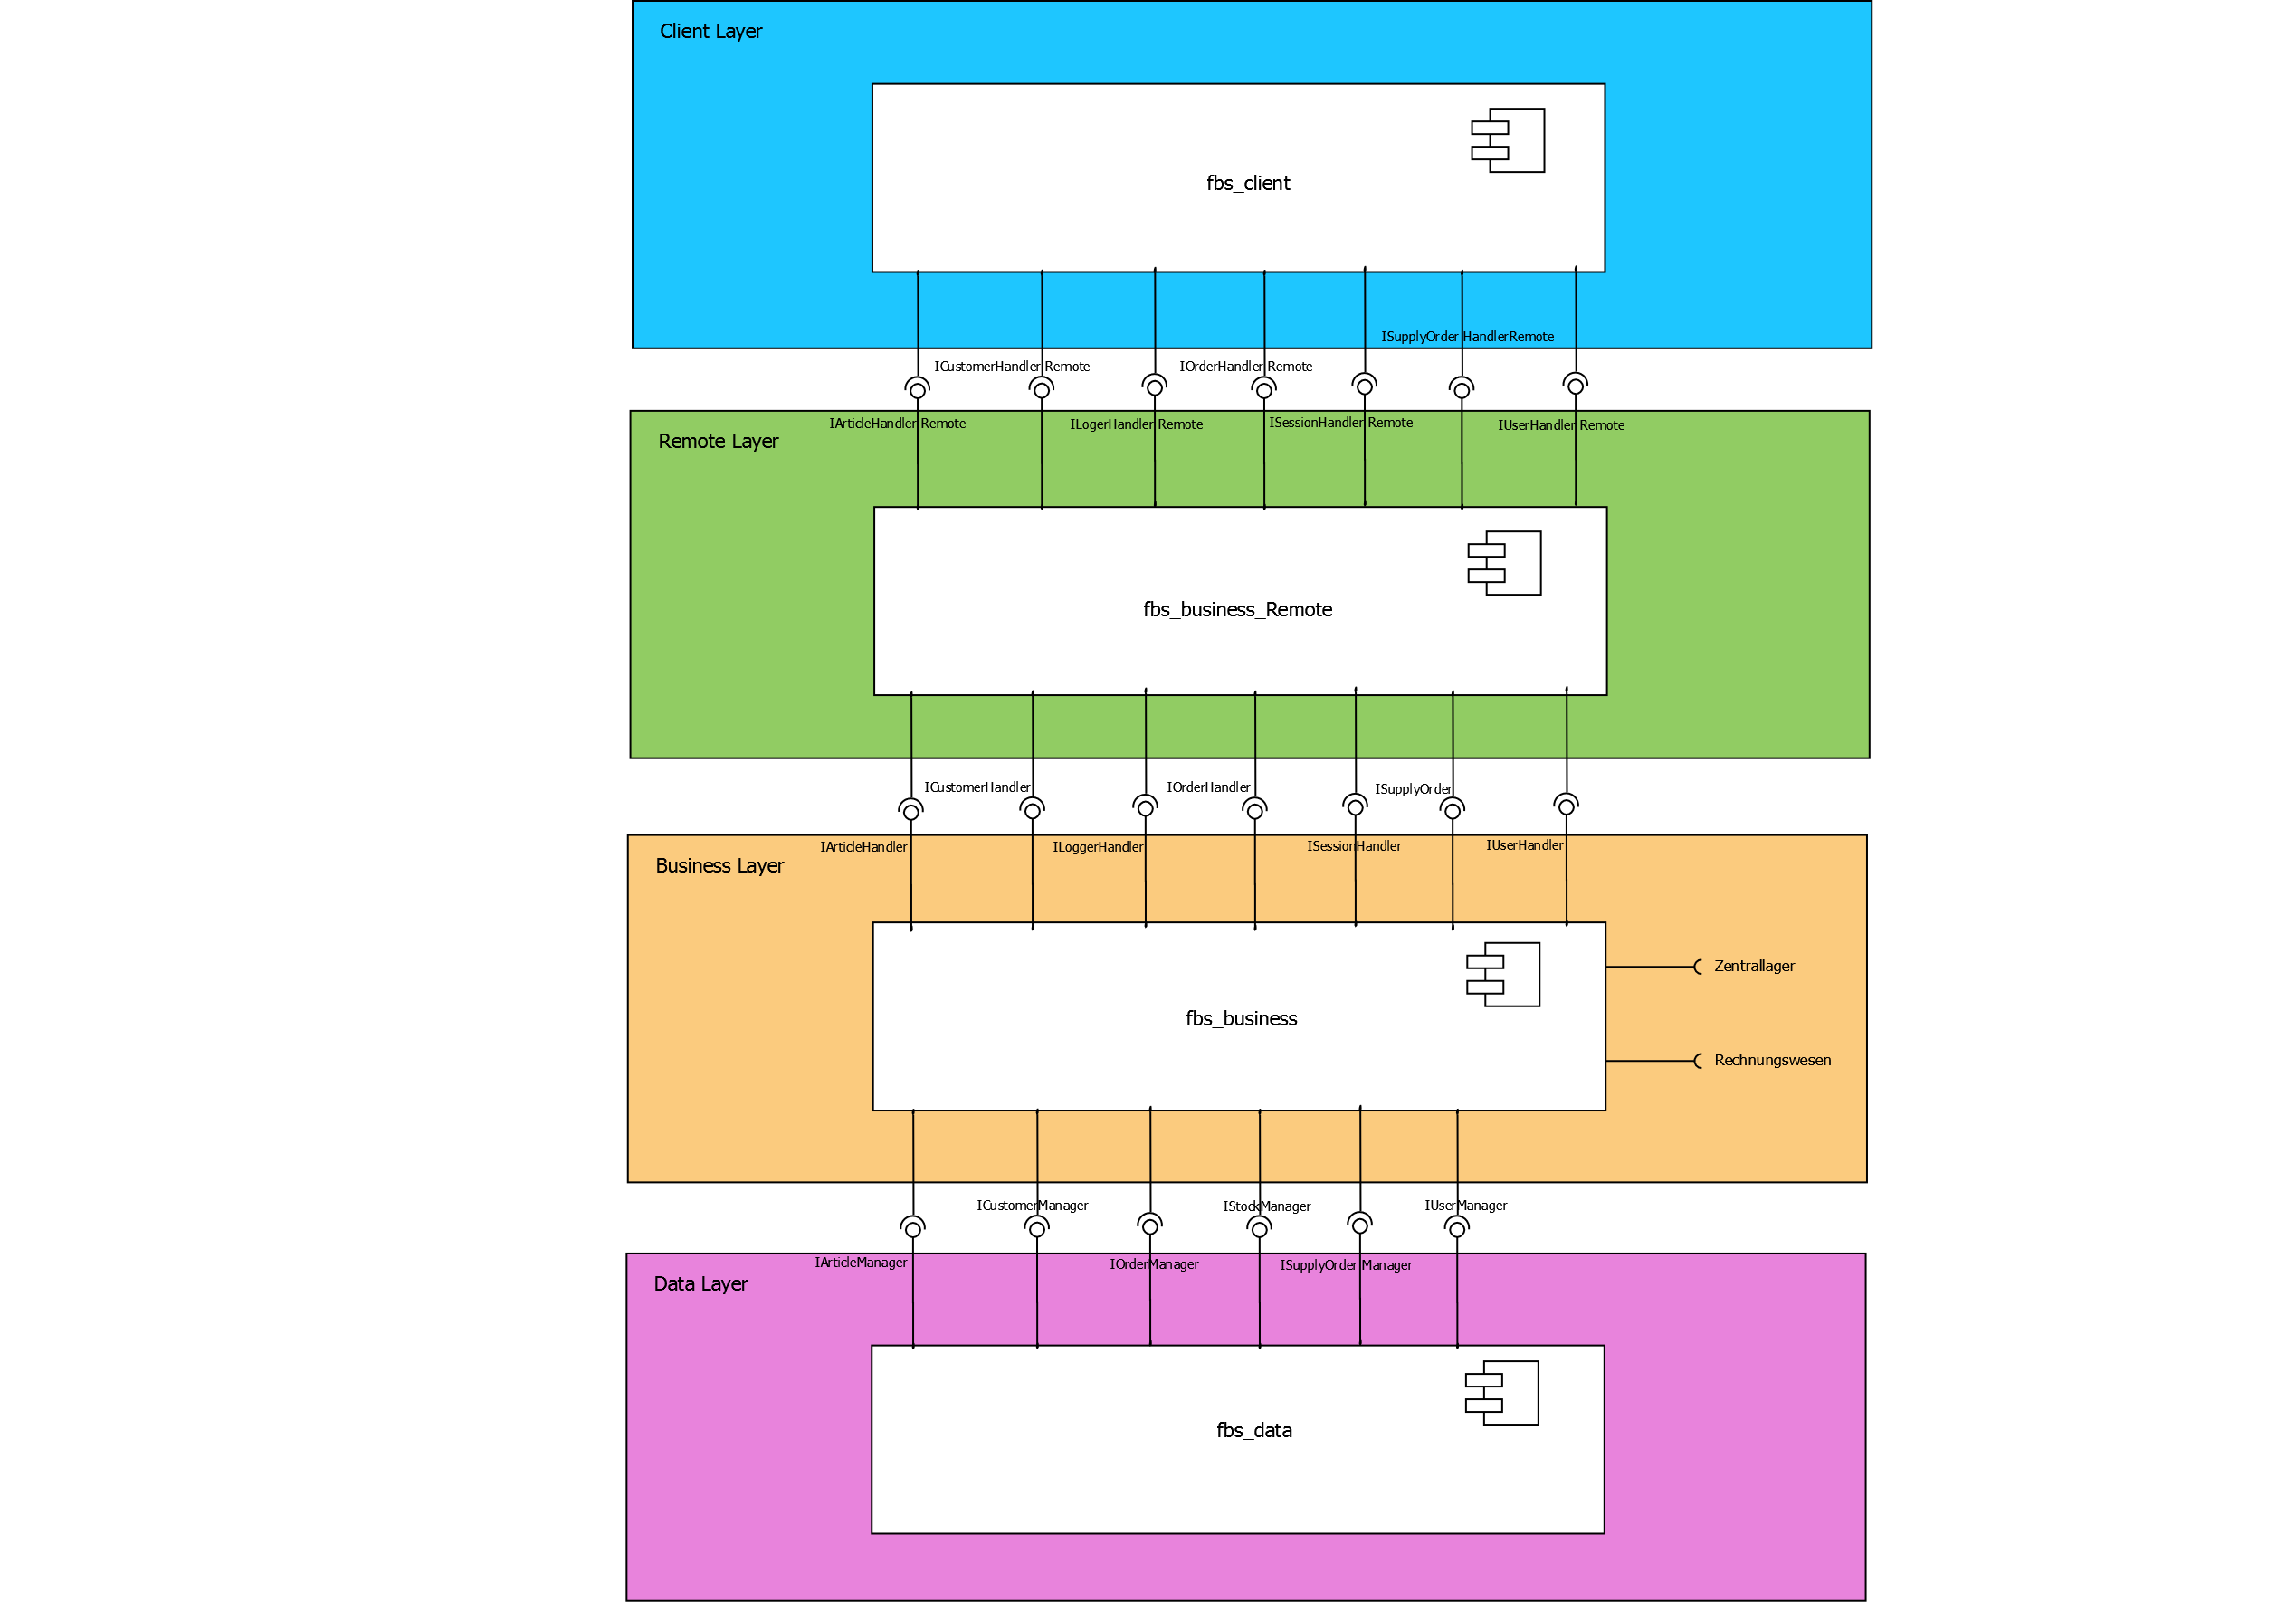
\includegraphics[width=1.0\linewidth]{Images/Schnittstellen}
	\caption{Schnittstellen}
	\label{fig:schnittstellen}
\end{figure}

\subsubsection{Model}
TODO Severin

\subsubsection{Client <-> Business-Remote}
Der Client-Layer ist generell als MVC implementiert. Der Controller fordert bei Aktionen des Benutzers jeweils die nachgefragten Informationen über die Remote-Schicht an, und sendet neue und geänderte Bestellungen über die definierten Schnittstellen zur Remote-Schicht.
Der Client-Layer strukturiert die erhaltenen Daten in einem eigenen Model transient ab.
TODO Klassendiagramme hinzufügen, eventuell Sequenz-Diagram

Speziell ist das User- und Session-Management. Der User erhält auf Basis der über die Login-Schnittstelle erhaltenen Benutzergruppe seine Berechigung zugewiesen. Diese Zuweisung wird im Singelton-Pattern des Users abgespeichert.
Das Singleton-Pattern wird dabei benötigt, um den Kontext des Benutzers auf Business-Ebene zu prüfen.
TODO Klassendiagram hinzufügen

Die Kontext-Prüfung wird dabei über eine dedizierte Schnittstelle zu Beginn jedes Aufrufes eingeleitet. So werden ungültige Aufrufe verhindert.
TODO Klassendiagramme Hnzufügen

Der Login-Prozess der Applikation entscheidet auf Basis der erhaltenen Benutzergruppe, welche Ansicht der jeweilige Benutzer erhält. Diese Entscheidung ist dabei über ein Strategy-Pattern implementiert. 
TODO Klassendiagramme Hnzufügen

Die Implementation des Client-Layers beruht auf JavaFX, bzw. FXML. Diese Implementation erzwingt den Einsatz von Observable-Objekten.

Der Client ist stark von der Remote-Schicht der Business-Logik abhängig. Es ist nicht gedacht, dass der Client-Layer für andere Applikationen verwendet wird.


\subsubsection{Business-Remote <-> Business-Core}
TODO Marco
\subsubsection{Business-Core <-> Data}
TODO Marco \&Tobias


\section{Environment-Anforderungen}
%-------------------
% Environment
%-------------------
% !TEX root = Dokumentation_SysSpec.tex
\subsection{}

todo

\section{Ausblick}
%-------------------
% AUsblick/Angedachte Verbesserungen
%-------------------
% !TEX root = Dokumentation_SysSpec.tex
\subsection{Robustheit}
\begin{itemize}
	\item Ausfälle von Umsystemen abfangen.
	\item Datentyp-Mismatch zwischen Applikation und Datenbank abfangen (Overflows durch unterschiedliche Längendefinition)
\end{itemize}

\subsection{Performance \& Skalierung}
\begin{itemize}
	\item Datenbank-Notifications, wenn Datenbank erweitert werden muss (bspw durch max. Anzahl möglicher Bestellungen)
\end{itemize}

\subsection{Sicherheit}
\begin{itemize}
	\item Einsatz von 2-Faktor-Authentifizierung durch EInbindung von Open-Source-OTP-Software, bspw. Google Authenticator oder Microsoft Authenticator
	\item Verschlüsselung der Applikationsdaten (Stufe Datenbank) und der übertragenene Daten
	\item Applikation, Datenbank und Periphere Systeme prüfen die Identität der Umsysteme, bspw über Zertifikate.
	\item Applikation darf nur "lokale" Aufrufe ausführen. Sicherstellung, dass Applikation nicht über das Internet, sondern üer Unternehmens-Netzwerke kommuniziert (VPN-Tunnel, Trusted Networks)
	\item Usersessions mit dediziertem Sessionmanagement (bspw. Cookies) lösen
\end{itemize}

\subsection{Erweiterungen \& Features}
\begin{itemize}
	\item Anbindung einer zentralen Benutzerverwaltung (Applikationsbenutzer) wie AD
	\item Anbindung einer zentralen Kundenverwaltung zum Vermeiden von Redundanzen mit Rechnungswesen. Führt zu klarer Trennung von Aufgabenbereichen der Applikation.
	\item Einbindung einer zentralen Log-Infrastruktur wie Syslog
	\item Einbindung von kritischen Events für SIEM-Systeme
\end{itemize}

\end{document}